\section{Experimental Inventory and Implementation}
\label{app:inventory}
Table~\ref{tab:inventory} distinguishes new model training from historical reference reuse and separate checkpoint checks. The three completed selection studies train 238 new models and execute 15,232 new policy-evaluation episodes in total. The scoring diagnostic generates no actions and performs no optimizer updates. WebShop base calibration adds 64 train-only episodes. These counts are not pooled as independent learning observations.

\begin{table}[h]
\centering
\caption{Completed study inventory. Additional references and conditional repeats are excluded from primary selection means.}
\label{tab:inventory}
\small
\begin{tabular}{lrrl}
\toprule
Study & New models & New episodes & Primary design / additional checks\\
\midrule
Complete pass vs.\ replay & 68 & 4,352 & 64 primary + 4 repeats\\
Task matching & 70 & 4,480 & 64 primary + 4 repeats + 2 references\\
Task/action matching & 100 & 6,400 & 96 primary + 4 repeats\\
Stored-checkpoint reevaluation & 0 & 128 & 2 checkpoints, original configurations\\
Uniform scoring diagnostic & 0 & 0 & 1,194 forwards; 853 distinct inputs\\
WebShop base calibration & 0 & 64 & 32 shared goals, two public prompts\\
\bottomrule
\end{tabular}
\end{table}

\begin{table}[h]
\centering
\caption{Shared configuration for the controlled selection studies.}
\label{tab:config}
\small
\begin{tabular}{ll}
\toprule
Parameter & Value\\
\midrule
Backbone & Qwen3-4B-Instruct-2507, fixed revision\\
Revision & \texttt{cdbee75f17c01a7cc42f958dc650907174af0554}\\
Training precision / adaptation & BF16 / LoRA\\
LoRA rank / alpha / dropout & 16 / 32 / 0.05\\
Trainable projections & \texttt{q\_proj}, \texttt{k\_proj}, \texttt{v\_proj}, \texttt{o\_proj}\\
Learning rate / weight decay & $10^{-4}$ / 0\\
Warmup ratio / maximum sequence & 0.05 / 2,048 tokens\\
Microbatch / gradient accumulation & 1 example / 4 microbatches\\
Updates / sample presentations & 192 / 768\\
Distinct task/content budget (selection) & 256 per model\\
Evaluation families & 32 cooling + 32 heating tasks, equal weights\\
Environment seed / temperature / batch & 11 / 0 / 8\\
Collection-specific guidance & Removed during evaluation\\
Official final evaluation sets & Unopened\\
\bottomrule
\end{tabular}
\end{table}

\smallpara{Checkpoint composition.}
The inherited evaluation path serves a trained A adapter plus an untrained B adapter at optimizer step zero. The B adapter has zero effect on the base prediction at initialization, but it remains part of the serialized composition. Audits verify the base revision, A-weight identity, zero-B reference identity, and full composition revision. We do not silently reinterpret the artifact as an independently served A-only checkpoint. The symbol $\Delta(\phi)$ in Eq.~\eqref{eq:sft} denotes the trainable A-adapter update.

\smallpara{Consumption and budget accounting.}
Presentations, processed input tokens, supervised target tokens, initialized parameters, trained weights, schedules, and physical GPU assignments are recorded separately. Time accounting includes model loading, training, serving, diagnostics, interrupted attempts, and shutdown. The complete task/action study uses 14.663 cumulative GPU-hours with a fixed 18-hour cap. No direction-dependent early stop, seed replacement, or queue extension is used.

\clearpage
\section{Initialization-Level Results and Conditional Repeats}
\label{app:seeds}
Table~\ref{tab:seeds} reports each initialization-level mean over four sampling recipes for the completed task/action comparison. Initialization 404 has a zero API difference even though its individual cells include positive and negative values. Its presence prevents a claim that every API initialization favors random selection. Conditional repeats in Table~\ref{tab:repeats} use the same initialization, recipe, and physical GPU as their originals, with different final trained parameters.

\begin{table}[h]
\centering
\caption{Task/action matching: low NLL minus random, in percentage points.}
\label{tab:seeds}
\begin{tabular}{rrr}
\toprule
Initialization/dropout seed & API & Generic\\
\midrule
\InitializationRows
\bottomrule
\end{tabular}
\end{table}

\begin{figure}[h]
\centering
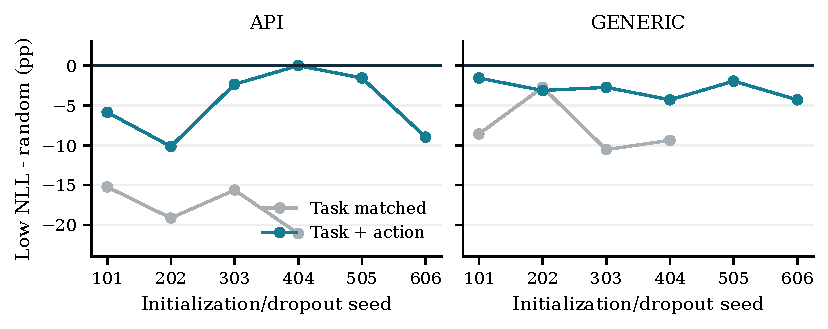
\includegraphics[width=\linewidth]{initialization-effects.pdf}
\caption{\textbf{Initialization-level effects.} Each point averages four sampling recipes. Task matching has four initialization levels; task/action matching has six. The figure shows descriptive crossed-seed outcomes and does not encode confidence intervals. Differences between curves also reflect changed content support and selection strength.}
\label{fig:initialization}
\end{figure}

\begin{table}[h]
\centering
\caption{Four prespecified task/action-study conditional repeats. Initialization 101 and recipe 101 throughout. Success rates are percentages.}
\label{tab:repeats}
\begin{tabular}{llrrr}
\toprule
Source & Policy & Original & Repeat & Change (pp)\\
\midrule
API & Random & 31.250 & 31.250 & 0.000\\
API & Low NLL & 34.375 & 29.688 & $-4.688$\\
Generic & Random & 4.688 & 6.250 & $+1.562$\\
Generic & Low NLL & 4.688 & 3.125 & $-1.562$\\
\bottomrule
\end{tabular}
\end{table}

\clearpage
\section{Scoring Geometry and Selection Sensitivity}
\label{app:scoring}
The completed diagnostic freezes 32 stress inputs: 16 selected for large recorded cache spans and 16 selected by content hash from the remainder. It evaluates canonical unpadded inputs with explicit positions and a fixed logits window, a canonical repeat, unpadded default positions, a dynamic logits window, and four padded conditions. It separately evaluates FP32 references, four direct supervised-loss checks, 392 original-layout replay observations, and uniform BF16 scores for all 853 distinct message inputs. The 1,194 forwards are fully accounted for; no retries, generated tokens, training updates, or teacher calls are included.

Canonical repeat, unpadded default-position, and dynamic-window conditions match canonical scores exactly on the 32 stress inputs. Across padded conditions, mean absolute score deviations range from 0.0362 to 0.0603 nat/token. BF16 versus FP32 deviation has mean 0.0396 and maximum 0.1630, with rank correlation 0.9857 on the selected inputs. Original batch layouts reproduce their original cached values exactly. These results quantify the instrument on the prespecified stress set; they do not estimate population error rates.

\begin{figure}[htbp]
\centering
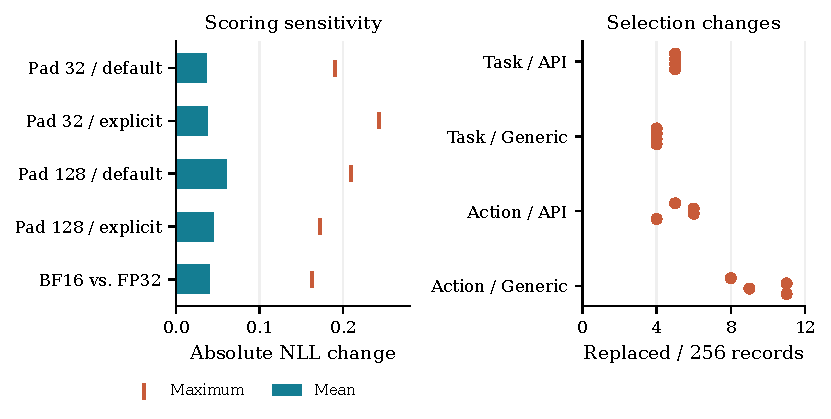
\includegraphics[width=\linewidth]{scoring-diagnostic.pdf}
\caption{\textbf{Completed scoring diagnostic.} Left: numerical layout sensitivity on the deliberately selected stress set. Right: content replacement after complete uniform rescoring, with each point a frozen selection recipe. The comparison changes the scoring procedure, not the training outcomes; the canonical-score retraining study is separate and ongoing.}
\label{fig:scoring}
\end{figure}

\begin{table}[h]
\centering
\caption{Content records replaced out of 256 after uniform rescoring. Columns are sampling-recipe seeds. Original recipes are regenerated exactly before replacement is counted.}
\label{tab:replacement}
\begin{tabular}{llrrrr}
\toprule
Control & Source & 101 & 202 & 303 & 404\\
\midrule
Task matched & API & 5 & 5 & 5 & 5\\
Task matched & Generic & 4 & 4 & 4 & 4\\
Task/action matched & API & 5 & 6 & 6 & 4\\
Task/action matched & Generic & 8 & 11 & 9 & 11\\
\bottomrule
\end{tabular}
\end{table}

\smallpara{Ongoing canonical-score replication.}
A separate freeze specifies 96 newly trained models, six initialization/dropout seeds, four recipes, two sources, and two policies, at the same 192-update budget and with the same 64 development tasks. Random indices must remain identical to the previous reference; low-NLL schedules use the completed uniform scores. Both policies are retrained, with an 18 cumulative GPU-hour cap. This study is running as of the manuscript's evidence cutoff. No interim outcome enters the completed-result comparisons in this paper.

\clearpage
\section{Second-Environment Base Calibration}
\label{app:webshop}
The WebShop pilot uses the full product/search backend and the pinned base checkpoint without an adapter. It evaluates 32 shared training goals under public ReAct and Act-only prompt ports, with at most 14 model decisions per episode and at most 100 output tokens per decision. All decisions, including thoughts and invalid controls, consume the episode budget. The backend is not queried through the ALFWorld training model servers.

\begin{table}[h]
\centering
\caption{Train-only WebShop calibration. Model-output errors are distinct from transport errors; all requests complete. This is not a post-SFT selection comparison.}
\label{tab:webshop}
\small
\begin{tabular}{lrr}
\toprule
Metric & ReAct & Act-only\\
\midrule
Goals solved / evaluated & 5/32 & 6/32\\
Success (\%) & 15.625 & 18.750\\
Mean partial score & 0.4125 & 0.4380\\
Model requests & 247 & 216\\
Physical actions & 86 & 91\\
Thought decisions & 78 & 38\\
Invalid format / invalid control & 24 / 59 & 10 / 77\\
Episodes exhausting decision budget & 10 & 10\\
Transport errors & 0 & 0\\
\bottomrule
\end{tabular}
\end{table}

\begin{figure}[htbp]
\centering
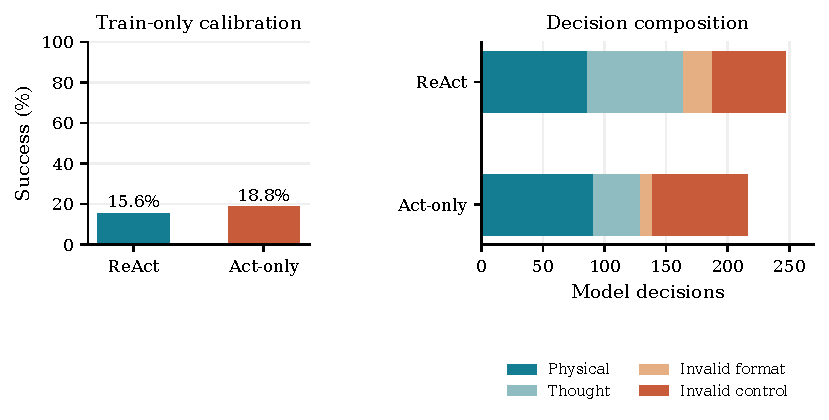
\includegraphics[width=\linewidth]{webshop-calibration.pdf}
\caption{\textbf{WebShop starting-point calibration.} Two public prompt ports on the same 32 training goals. Success-count differences of one goal do not establish prompt superiority. The composition of model decisions exposes substantial invalid-format/control behavior and informs a future learning protocol.}
\label{fig:webshop}
\end{figure}

Across both prompts the pilot records 703,520 input and 15,844 output tokens, 463 completed requests, and 243.564 GPU seconds. Teacher calls, official evaluation episodes, and optimizer updates are zero. A second-environment \emph{learning} comparison must still fix the candidate pool, selection unit, training budget, common executor, and fresh task protocol.

\clearpage
\section{Retained Baseline and Evidence Boundaries}
\label{app:baseline}
The API-versus-ReAct source study is distinct from the API/Generic pools used in the controlled selection experiments. Both source collectors make 144 attempts using the same base student. The API condition uses cached guidance from public resets; ReAct uses public examples and reasoning/action interaction. The conditions also differ in format and thought mechanism, so that comparison is a pipeline comparison, not an isolated teacher-card intervention.

Common-success matching uses 58 paired successful task/environment-seed cases and yields 452 eligible action labels per source. At 256 A-training presentations, the raw adaptation-AUC difference is $-3.564$ points. The full eligible corpora instead contain 726 API and 981 ReAct labels. A prepared 1,024-presentation schedule visits each complete corpus at least once, but its formal source-comparison study has not been executed. The old negative result remains part of the evidence and is not replaced by the within-pool selection analysis.

\smallpara{Scope relative to existing selectors.}
The implemented low-NLL policy selects action examples and uses ordinary supervised target loss. SmartAD additionally selects complete correct teacher trajectories and applies segment weighting; LESS uses target demonstrations and optimizer-aware gradient features; Rho-1 uses a reference-based token criterion. These methods require distinct implementation and cost accounting. No scores from incompatible published benchmark splits are inserted into our result table.

\smallpara{Provenance and reproducibility.}
The source bundle contains the full \LaTeX{} manuscript, editable TikZ diagrams, vector result figures, a BibTeX database, a figure/table generation script, and a hash-bound evidence manifest. Completed results are regenerated from local audited JSON reports. Raw goals, messages, scoring journals, credentials, and adapter weights are not included in the manuscript package. The official NeurIPS style is preserved byte-for-byte with its download source and SHA256. The document uses preprint mode and does not claim acceptance or submission to a particular venue.

\smallpara{Responsible reporting.}
The experiments involve simulated tasks and no new human-subject data. We use existing models, environment data, and baseline resources under their original terms. We make no real-robot, real-purchase, safety, recursive self-improvement, or state-of-the-art claim. Authors must complete venue-specific disclosures, anonymity checks, and the final checklist before an actual submission.
